\subsection{Conics over the Reals}

\begin{tcolorbox}[title=Problem 1, breakable]
    \[P(x,y) = y - x^2, \quad C = \{(x, y) \in \mathbb{R}^2 \mid P(x, y) = 0\}.\]
    Show that for any $(x, y) \in C$, we also have 
    \[(-x, y) \in C.\]
    Thus the curve is symmetric about the y-axis.
\end{tcolorbox}

\begin{proof}
    Let $(x, y) \in C$.
    Then $P(x, y) = y - x^2 = 0$.
    Let $x' = -x$ and note that $(-x)^2 = x^2$.
    Thus
    \[
        P(-x, y) = y - (-x)^2 = y - x^2 = 0.
    \]
    Thus $(-x, y) \in C$.
\end{proof}

\begin{tcolorbox}[title=Problem 2, breakable]
    \[P(x,y) = y - x^2, \quad C = \{(x, y) \in \mathbb{R}^2 \mid P(x, y) = 0\}.\]
    Show that if $(x, y) \in C$, then we have $y \ge 0$.
\end{tcolorbox}

\begin{proof}
    Suppose $(x, y) \in C$.
    Then 
    \[P(x, y) = y - x^2 = 0 \iff y = x^2 \ge 0.\]
    Thus $y \ge 0$.
\end{proof}

\begin{tcolorbox}[title=Problem 3, breakable]
    \[P(x,y) = y - x^2, \quad C = \{(x, y) \in \mathbb{R}^2 \mid P(x, y) = 0\}.\]
    Show that for every $y \ge 0$, there is a point $(x, y) \in C$
    with this $y$-coordinate. Now, for points $(x, y) \in C$, show that if 
    $y$ goes to infinity, then one of the corresponding $x$-coordinates also 
    approaches infinity while the other corresponding $x$ coordinate must approach negative 
    infinity.
\end{tcolorbox}

\begin{proof}
    Let $y \in \mathbb{R}$ such that $y \ge 0$.
    Let $x = \sqrt{y} \in \mathbb{R}$.
    Then
    \[
        y - x^2 = y - (\sqrt{y})^2 = y - y = 0.
    \]
    Thus $(x, y) = (\sqrt{y}, y) \in C$.

    Now suppose $y \to \infty$.
    For points $(x, y) \in C$, we have
    \[
        y - x^2 = 0 \iff x = \pm \sqrt{y}.
    \]
    Since $y \to \infty$, we have $\sqrt{y} \to \infty$ and $-\sqrt{y} \to -\infty$.
    Thus one corresponding $x$-coordinate approaches infinity, while the other
    approaches negative infinity.
\end{proof}

\begin{tcolorbox}[title=Problem 4, breakable]
    Sketch the curve $C = \{(x, y) \in \mathbb{R}^2 \mid P(x, y) = 0\}$.
\end{tcolorbox}

\begin{center}
\begin{tikzpicture}[scale=0.9]
    % Axes
    \draw[->] (-3,0) -- (3,0) node[right] {$x$};
    \draw[->] (0,-1) -- (0,5) node[above] {$y$};

    % Parabola y = x^2
    \draw[domain=-2:2, smooth, thick, blue] plot (\x, {\x*\x});

    % Labels
    \node at (2,4) {$y = x^2$};
\end{tikzpicture}
\end{center}


\begin{tcolorbox}[title=Problem 5, breakable]
    \[C = \left\{(x, y) \in \mathbb{R}^2 \mid \frac{x^2}{4} + \frac{y^2}{9} - 1 = 0 \right\}.\]
    Show that if $(x, y) \in C$, then the three points $(-x, y), (x, -y), (-x, -y)$ are also on $C$.
    Thus the curve $C$ is symmetric about both the $x$- and $y$-axes.
\end{tcolorbox}

\begin{proof}
    Let $(x, y) \in \mathbb{R}^2$.
    Suppose $\frac{x^2}{4} + \frac{y^2}{9} - 1 = 0$.
    Notice that $x^2 = (-x)^2$ and $y = (-y)^2$. Then 
    \[\frac{x^2}{4} + \frac{y^2}{9} - 1 = \frac{(-x)^2}{4} + \frac{y^2}{9} - 1 
                                        = \frac{x^2}{4} + \frac{(-y)^2}{9} - 1 
                                        = \frac{(-x)^2}{4} + \frac{(-y)^2}{9} - 1 = 0.\]
    Thus $(-x, y), (x, -y), (-x, -y) \in C$.
\end{proof}

\begin{tcolorbox}[title=Problem 6, breakable]
    \[C = \left\{(x, y) \in \mathbb{R}^2 \mid \frac{x^2}{4} + \frac{y^2}{9} - 1 = 0 \right\}.\]
    Show that for every $(x, y) \in C$, we have $|x| \le 2$ and $|y| \le 3$.
\end{tcolorbox}

\begin{proof}
    Let $(x, y) \in C$.
    Then 
    \[\frac{x^2}{4} + \frac{y^2}{9} - 1 = 0 \iff 9 x^2 + 4 y^2 - 36 = 0 \iff 9x^2 = -4 y^2 + 36 \iff |x| = \sqrt{\frac{-4}{9} y^2 + 4} \le \sqrt{4} = 2.\]
    Similarly 
    \[9x^2 + 4 y^2 - 36 = 0 \iff |y| = \sqrt{\frac{-9}{4} x^2 + 9} \le \sqrt{9} = 3.\]
\end{proof}

\begin{tcolorbox}[title=Problem 7, breakable]
    Sketch 
    \[C = \left\{(x, y) \in \mathbb{R}^2 \mid \frac{x^2}{4} + \frac{y^2}{9} - 1 = 0 \right\}.\]
\end{tcolorbox}

\begin{center}
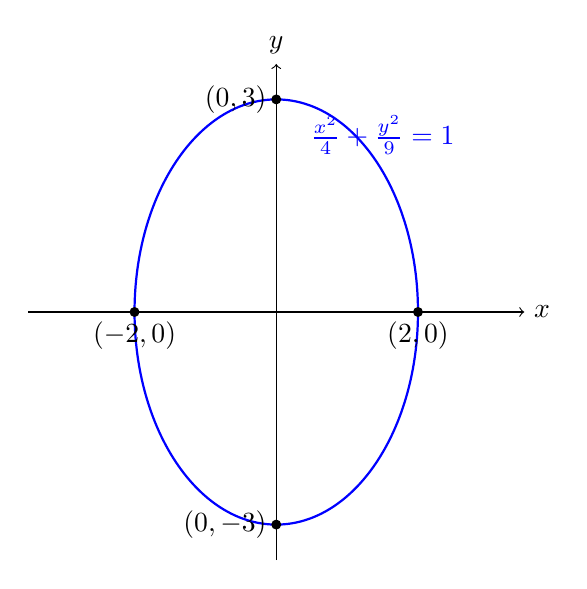
\begin{tikzpicture}[scale=0.9]
    % Axes
    \draw[->] (-3.5,0) -- (3.5,0) node[right] {$x$};
    \draw[->] (0,-3.5) -- (0,3.5) node[above] {$y$};

    % Ellipse: x^2/4 + y^2/9 = 1
    \draw[thick, blue] (0,0) ellipse (2 and 3);

    % Mark key points
    \foreach \x in {-2,2} \fill (\x,0) circle (2pt) node[below] {$(\x,0)$};
    \foreach \y in {-3,3} \fill (0,\y) circle (2pt) node[left] {$(0,\y)$};

    % Label the curve
    \node[blue] at (1.5,2.5) {$\frac{x^2}{4} + \frac{y^2}{9} = 1$};
\end{tikzpicture}
\end{center}

\begin{tcolorbox}[title=Problem 8, breakable]
    \[C = \left\{(x, y) \in \mathbb{R}^2 \mid x^2 - y^2 - 4 = 0\right\}.\]
    Show that if $(x, y) \in C$, then the three points $(-x, y), (x, -y)$, and $(-x, -y)$
    are also on $C$. Thus the curve $C$ is also symmetric about the $x-$ and $y$-axes.
\end{tcolorbox}

\begin{proof}
    Let $(x, y) \in \mathbb{R}^2$.
    Suppose $x^2 - y^2 - 4 = 0$.
    Notice that $x^2 = (-x)^2$ and $y = (-y)^2$. Then 
    \[x^2 - y^2 - 4 = (-x)^2 - y^2 = x^2 - (-y)^2 = (-x)^2 - (-y)^2 = 0.\]
    Thus $(-x, y), (x, -y), (-x, -y) \in C$.
\end{proof}

\begin{tcolorbox}[title=Problem 9, breakable]
    \[C = \left\{(x, y) \in \mathbb{R}^2 \mid x^2 - y^2 - 4 = 0\right\}.\]
    Show that if $(x, y) \in C$, then we have $|x| \ge 2$.
\end{tcolorbox}

\begin{proof}
    Let $(x, y) \in \mathbb{R}^2$.
    Suppose $x^2 - y^2 - 4 = 0$.
    Then 
    \[x^2 - y^2 - 4 = 0 \iff x^2 = y^2 + 4 \iff |x| = \sqrt{y^2 + 4} \ge \sqrt{4} = 2.\]
\end{proof}

\begin{tcolorbox}[title=Problem 10, breakable]
    \[C = \left\{(x, y) \in \mathbb{R}^2 \mid x^2 - y^2 - 4 = 0\right\}.\]
    Show that the curve $C$ is unbounded in the positive 
        and negative $x$-directions and also unbounded in the 
        positive and negative $y$-directions.
\end{tcolorbox}

\begin{proof}
    First notice
    \[
        x^2 - y^2 - 4 = 0 
        \iff x^2 = y^2 + 4 
        \iff x = \pm \sqrt{y^2 + 4}
        \iff y = \pm \sqrt{x^2 - 4}.
    \]
    As $y \to \infty$, we have $x = \pm \sqrt{y^2 + 4} \to \infty$ and $-\infty$.
    Similarly, as $x \to \infty$, we have $y = \pm \sqrt{x^2 - 4} \to \infty$ and $-\infty$.
\end{proof}


\begin{tcolorbox}[title=Problem 11, breakable]
    Sketch 
    \[C = \left\{(x, y) \in \mathbb{R}^2 \mid x^2 - y^2 - 4 = 0\right\}.\]
\end{tcolorbox}

\begin{center}
\begin{tikzpicture}[scale=0.8]
    % Axes
    \draw[->] (-6,0) -- (6,0) node[right] {$x$};
    \draw[->] (0,-5) -- (0,5) node[above] {$y$};

    % Hyperbola x^2 - y^2 = 4
    \draw[domain=-5:-2, smooth, thick, blue] 
        plot (\x, {sqrt(\x*\x - 4)});
    \draw[domain=-5:-2, smooth, thick, blue] 
        plot (\x, {-sqrt(\x*\x - 4)});
    \draw[domain=2:5, smooth, thick, blue] 
        plot (\x, {sqrt(\x*\x - 4)});
    \draw[domain=2:5, smooth, thick, blue] 
        plot (\x, {-sqrt(\x*\x - 4)});

    % Asymptotes y = ±x
    \draw[dashed] (-5,-5) -- (5,5);
    \draw[dashed] (-5,5) -- (5,-5);

    % Label
    \node[blue] at (3.5,2.5) {$x^2 - y^2 = 4$};
\end{tikzpicture}
\end{center}

\begin{tcolorbox}[title=Problem 12, breakable]
    Sketch the graph of each of the following conics in 
        $\mathbb{R}^2$.
    Identify which are parabolas, ellipses, or Hyperbola.
    \begin{enumerate}
        \item $V(x^2 - 8y)$.
        \item $V(x^2 + 2x - y^2 - 3y - 1)$.
        \item $V(4x^2 + y^2)$.
        \item $V(3x^2 + 3y^2 - 75)$.
        \item $V(x^2 - 9y^2)$.
        \item $V(4x^2 + y^2 - 8)$.
        \item $V(x^2 + 9y^2 - 36)$.
        \item $V(x^2 - 4 y^2 - 16)$.
        \item $V(y^2 - x^2 - 9)$.
    \end{enumerate}
\end{tcolorbox}

\textbf{Solution (1):}
Parabola.
\begin{figure}[h!]
    \centering
    \includegraphics[width=0.3\textwidth]{images/chapter1/1.png}
\end{figure}

\textbf{Solution (2):}
Hyperbola.
\begin{figure}[h!]
    \centering
    \includegraphics[width=0.3\textwidth]{images/chapter1/2.png}
\end{figure}

\textbf{Solution (3):}
Point.

\textbf{Solution (4):}
Ellipse.
\begin{figure}[h!]
    \centering
    \includegraphics[width=0.3\textwidth]{images/chapter1/4.png}
\end{figure}

\textbf{Solution (5):}
Two lines.
\begin{figure}[h!]
    \centering
    \includegraphics[width=0.3\textwidth]{images/chapter1/5.png}
\end{figure}

\textbf{Solution (6):}
Ellipse.
\begin{figure}[h!]
    \centering
    \includegraphics[width=0.3\textwidth]{images/chapter1/6.png}
\end{figure}

\textbf{Solution (7):}
Ellipse.
\begin{figure}[h!]
    \centering
    \includegraphics[width=0.3\textwidth]{images/chapter1/7.png}
\end{figure}

\textbf{Solution (8):}
Hyperbola.
\begin{figure}[h!]
    \centering
    \includegraphics[width=0.3\textwidth]{images/chapter1/8.png}
\end{figure}

\textbf{Solution (9):}
Hyperbola.
\begin{figure}[h!]
    \centering
    \includegraphics[width=0.3\textwidth]{images/chapter1/9.png}
\end{figure}

\begin{tcolorbox}[title=Problem 13, breakable]
    Express the polynomial $P(x, y) = ax^2 + bxy + cy^2 + dx + ey + h$ in the form
    \[P(x, y) = Ax^2 + Bx + C,\]
    where $A, B$, and $C$ are polynomials in $y$. What are $A, B$, and $C$?
\end{tcolorbox}

\begin{proof}
    Let $A = a, B = by + d$, and $C = cy^2 + ey + h$.
    Notice 
    \[
    ax^2 + bxy + cy^2 + dx + ey + h
    = a x^2 + bxy + dx + cy^2 + ey + h
    = a x^2 + (by + d)x + (cy^2 + ey + h)
    = Ax^2 + Bx + C.
    \]
\end{proof}

\begin{tcolorbox}[title=Problem 14, breakable]
    Treating $P(x, y) = ax^2 + bxy + cy^2 + dx + cy + h$ as a polynomial
    in the variable $x$, show that the discriminant is 
    \[\triangle_x (y) = (b^2 - 4ac)y^2 + (2bd - 4ae)y + (d^2 - 4ah).\]
\end{tcolorbox}

\begin{proof}
    From Problem 13 we have $A = a, B = by + d$, and $C = cy^2 + ey + h$.
    Then 
    \[
    \triangle_x (y) = B^2 - 4AC
    = (by + d)^2 - 4a(cy^2 + ey + h)
    = (b^2 - 4ac)y^2 + (2bd - 4ae)y + (d^2 - 4ah).
    \]
\end{proof}

\begin{tcolorbox}[title=Problem 15, breakable]
    \begin{enumerate}
        \item Suppose $\triangle_x (y_0) < 0$. Explain why there is no point on $V(p)$ whose $y$-coordinate is $y_0$.
        \item Suppose $\triangle_x (y_0) = 0$. Explain why there is exactly one point on $V(P)$ whose $y$-coordinate is $y_0$.
        \item Suppose $\triangle_x (y_0) > 0$. Explain why there are exactly two points on $V(P)$ whose $y$-coordinate is $y_0$.
    \end{enumerate}
\end{tcolorbox}

\textbf{Solution (a):} In $\mathbb{R}$, the square root is undefined for values $< 0$.

\textbf{Solution (b):} If $\triangle_x (y_0) = 0$, then $+\sqrt{B^2 - 4AC} = -\sqrt{B^2 - 4AC}$,  
so there is exactly one point on $V(P)$ whose $y$-coordinate is $y_0$.

\textbf{Solution (c):} If $\triangle_x (y_0) > 0$, then $+\sqrt{B^2 - 4AC} \ne -\sqrt{B^2 - 4AC}$,  
so there are exactly two points on $V(P)$ whose $y$-coordinate is $y_0$.

\begin{tcolorbox}[title=Problem 16, breakable]
    Suppose $b^2 - 4ac = 0$. Suppose further that $2bd - 4 ae > 0$.
    \begin{enumerate}
        \item Show that $\triangle_x (y) \ge 0$ if and only if $y \ge \frac{4 ah - d^2}{2bd - 4ae}$.
        \item Conclude that if $b^2 - 4ac = 0$ and $2bd - 4ae > 0$, then $V(P)$ is a parabola.
    \end{enumerate}
\end{tcolorbox}

\begin{proof}
    Suppose $\triangle_x (y) \ge 0$.
    Then 
    \begin{align*}
        \triangle_x (y) &= (b^2 - 4ac)y^2 + (2bd - 4ae)y + (d^2 - 4ah) \\
                        &= 0 y^2 + (2bd - 4 ae)y + (d^2 - 4ah).
    \end{align*}
    Therefore,
    \[
        (2bd - 4ae)y + (d^2 - 4ah) \ge 0.
    \]
    Since $2bd - 4ae > 0$, we have
    \[
        y \ge \frac{4ah - d^2}{2bd - 4ae}.
    \]
    Conversely, suppose $y \ge \frac{4ah - d^2}{2bd - 4ae}$.
    Then 
    \begin{align*}
        \triangle_x (y) &= (2bd - 4ae)y + (d^2 - 4ah) \\
                        &\ge (2bd - 4ae)\left(\frac{4ah - d^2}{2bd - 4ae}\right) + (d^2 - 4ah) \\
                        &= 0.
    \end{align*}
\end{proof}

\begin{proof}
    Suppose $b^2 - 4ac = 0$ and $2bd - 4ae > 0$.
    Then $\triangle_x (y) = (2bd - 4ae)y + (d^2 - 4ah)$.
    Now, $x = \frac{-B \pm \sqrt{B^2 - 4AC}}{2A}$.
    It is clear that $x$ is symmetrical, and since $y \ge \frac{4ah - d^2}{2bd - 4ae}$,
    $V(P)$ is a parabola.
\end{proof}


\begin{tcolorbox}[title=Problem 17, breakable]
    Suppose $b^2 - 4ac < 0$.
    \begin{enumerate}
        \item Show that one of the following occurs:
        \begin{enumerate}
            \item $\{y \mid \triangle_x (y) \ge 0\} = \emptyset$,
            \item $\{y \mid \triangle_x (y) \ge 0\} = \{y_o\}$,
            \item there exist real numbers $\alpha$ and $\beta$, $\alpha < \beta$, such that 
            \[\{y \mid \triangle_x (y) \ge 0\} = \{y \mid \alpha \le y \le \beta\}.\]
        \end{enumerate}
        \item Conclude that $V(P)$ is either emptyset, a point, or an ellipse.
    \end{enumerate}
\end{tcolorbox}

\begin{proof}
    Since $b^2 - 4ac < 0$, the graph of
    $\triangle_x(y)$ is a downward opening parabola in $y$.
    There are three cases, depending on the number of real zeros of $\triangle_x(y)$.
    \begin{enumerate}
        \item If $\triangle_x(y) < 0$ for all $y$, then
        \[
            \{y \mid \triangle_x(y) \ge 0\} = \emptyset.
        \]
        \item If $\triangle_x(y)$ has exactly one real zero $y_0$, then
        \[
            \{y \mid \triangle_x(y) \ge 0\} = \{y_0\}.
        \]
        \item If $\triangle_x(y)$ has two distinct real zeros $\alpha < \beta$, then
        \[
            \{y \mid \triangle_x(y) \ge 0\} = \{y \mid \alpha \le y \le \beta\}.
        \]
    \end{enumerate}
\end{proof}

\begin{proof}
    From part 1 the set of $y$ values is either empty, a single point, or a bounded interval, it follows that
        $V(P)$ is either empty, a point, or an ellipse.
\end{proof}


\begin{tcolorbox}[title=Problem 18, breakable]
    Suppose $b^2 - 4ac > 0$.
    \begin{enumerate}
        \item Show that one of the following occurs:
        \begin{enumerate}
            \item $\{y \mid \triangle_x (y) \ge 0\} = \mathbb{R}$ and $\triangle_x (y) \ne 0$,
            \item $\{y \mid \triangle_x (y) = 0\} = \{y_0\}$ and $\{y \mid \triangle_x (y) > 0\} = \{y \mid y \ne y_0\}$,
            \item there exist real numbers $\alpha$ and $\beta$, $\alpha < \beta$, such that 
            \[\{y \mid \triangle_x (y) \ge 0\} = \{y \mid y \le \alpha\} \cup \{y \mid y \ge \beta\}.\]
        \end{enumerate}
        \item If $\{y \mid \triangle_x (y)\} = \mathbb{R}$, show that $V(P)$ is a hyperbola opening left and right.
        \item If $\{y \mid \triangle_x (y) = 0\} = \{y_0\}$, show that $V(P)$ is two lines intersecting in a point.
        \item If there are two real numbers $\alpha$ and $\beta$, $\alpha < \beta$, such that 
        \[\{y \mid \triangle_x (y) \ge 0\} = \{y \mid y \le \alpha\} \cup \{y \mid y \ge \beta\},\]
        show that $V(P)$ is a hyperbola opening up and down.
    \end{enumerate}
\end{tcolorbox}

\begin{proof}
    Since $b^2 - 4ac > 0$, the graph of
    $\triangle_x(y)$ is an upward opening parabola in $y$.
    There are three cases, depending on the number of real zeros of $\triangle_x(y)$.
    \begin{enumerate}
        \item If $\triangle_x(y) > 0$ for all $y$, then
        \[
            \{y \mid \triangle_x(y) \ge 0\} = \mathbb{R}.
        \]
        \item If $\triangle_x(y)$ has exactly one real zero $y_0$, then
        \[
            \{y \mid \triangle_x (y) = 0\} = \{y_0\}
            \quad \text{and} \quad
            \{y \mid \triangle_x (y) > 0\} = \{y \mid y \ne y_0\}.
        \]
        \item If $\triangle_x(y)$ has two distinct real zeros $\alpha < \beta$, then
        \[
            \{y \mid \triangle_x (y) \ge 0\}
            = \{y \mid y \le \alpha\} \cup \{y \mid y \ge \beta\}.
        \]
    \end{enumerate}
\end{proof}

\begin{proof}
    Since $b^2 - 4ac > 0$, the graph of
    $\triangle_x(y)$ is an upward opening parabola in $y$.
    There are three cases, depending on the number of real zeros of $\triangle_x(y)$.
    \begin{enumerate}
        \item If $\triangle_x(y) > 0$ for all $y$, then
        \[
            \{y \mid \triangle_x(y) \ge 0\} = \mathbb{R}.
        \]
        \item If $\triangle_x(y)$ has exactly one real zero $y_0$, then
        \[
            \{y \mid \triangle_x (y) = 0\} = \{y_0\}
            \quad \text{and} \quad
            \{y \mid \triangle_x (y) > 0\} = \{y \mid y \ne y_0\}.
        \]
        \item If $\triangle_x(y)$ has two distinct real zeros $\alpha < \beta$, then
        \[
            \{y \mid \triangle_x (y) \ge 0\}
            = \{y \mid y \le \alpha\} \cup \{y \mid y \ge \beta\}.
        \]
    \end{enumerate}
\end{proof}

\begin{proof}
    Suppose $\{y \mid \triangle_x (y) \ge 0\} = \mathbb{R}$.
    Then for every $y$ there exist two real solutions for $x$, and $x$ is unbounded
    to the left and right. Since the equation is quadratic in $x$, the curve is
    symmetric in $x$.
    Thus $V(P)$ is a hyperbola opening left and right.
\end{proof}

\begin{proof}
    Suppose $\{y \mid \triangle_x (y) = 0\} = \{y_0\}$.
    Then for $y = y_0$ the equation has exactly one real solution for $x$, and for
    $y \ne y_0$ it has two real solutions. Since the equation is quadratic in $x$,
    $V(P)$ consists of two lines intersecting at a point.
\end{proof}

\begin{proof}
    Suppose there exist real numbers $\alpha$ and $\beta$, $\alpha < \beta$, such that
    \[
        \{y \mid \triangle_x (y) \ge 0\}
        = \{y \mid y \le \alpha\} \cup \{y \mid y \ge \beta\}.
    \]
    For $y \le \alpha$ or $y \ge \beta$, the equation has two real solutions in $x$.
    If $\alpha < y < \beta$ it has no real solutions. Thus $x$ is bounded for each
    $y$, but $y$ is unbounded above and below.
    Since the equation is quadratic in $x$, the curve is symmetric in $x$.
    Therefore $V(P)$ is a hyperbola opening up and down.
\end{proof}

\begin{tcolorbox}[title=Problem 19, breakable]
    Show that the discriminant of $A'y^2 + B'y + C' = 0$ is 
    \[\triangle_y (x) = (b^2 - 4ac)x^2 + (2be - 4cd)x + (e^2 - 4ch).\]
\end{tcolorbox}

\begin{proof}
    Here $A' = c$, $B' = bx + e$, and $C' = ax^2 + dx + h$. Then
    \[
        \triangle_y(x) = (B')^2 - 4 A' C'
        = (bx + e)^2 - 4 c (ax^2 + dx + h)
        = (b^2 - 4ac)x^2 + (2be - 4cd)x + (e^2 - 4ch).
    \]
\end{proof}

\subsection{Changes of Coordinates}

\begin{tcolorbox}[title=Problem 1, breakable]
    Show that the origin in the $xy$-coordinate system 
    agrees with the origin in the $uv$-system if and only if 
    $e = f = 0$. Thus the constants $e$ and $f$ describe 
    translations of the origin.
\end{tcolorbox}

\begin{proof}
    Suppose the $xy$-coordinate system agrees with the origin 
        of the $uv$-system.
    Then 
    \[u = 0 = a(0) + b(0) + e = e,\] 
    and 
    \[v = 0 = c(0) + d(0) + f = f.\]
    Thus $f = e = 0$.

    Conversely, suppose $e = f = 0$.
    Then 
    \[u = ax + by + e = ax + by + 0 = a(0) + b(0) = 0,\]
    and 
    \[v = cx + dy + f = cx + dy + 0 = c(0) + d(0) = 0.\]
    Thus the origin of the $xy$-coordinate system agrees with the 
        origin of the $uv$-system.
\end{proof}


\begin{tcolorbox}[title=Problem 2, breakable]
    Show that if $u = ax + by + e$ and $v = cx + dy + f$ 
        is a change of coordinates, then the inverse change of 
        coordinates is 
    \[x = \left( \frac{1}{ad - bc} \right) (du - bv) - \left( \frac{1}{ad - bc} \right) (de - bf).\]
    \[y = \left( \frac{1}{ad - bc} \right) (-cu + av ) - \left( \frac{1}{ad - bc} \right) (-ce + af).\]
\end{tcolorbox}

\begin{proof}
    We need to solve the two equations $u = ax + by + e$ and $v = cx + dy + f$ in two unknowns $x$ and $y$.
    Translating this to linear algebra, we have 
    \[
        \begin{bmatrix}
            a & b \\
            c & d
        \end{bmatrix}
        \begin{bmatrix}
            x \\ 
            y
        \end{bmatrix} = 
        \begin{bmatrix}
            u - e \\
            v - f
        \end{bmatrix}.
    \]
    Using Cramer's rule we see
    \[
        x = \frac{
            \begin{vmatrix} u - e & b \\ v - f & d \end{vmatrix}
        }{
            \begin{vmatrix} a & b \\ c & d \end{vmatrix}}
        = \frac{d(u-e) - b(v-f)}{ad - bc},
    \]
    \[
        y = \frac{
            \begin{vmatrix} a & u - e \\ c & v - f \end{vmatrix}
        }{
            \begin{vmatrix} a & b \\ c & d \end{vmatrix}}
        = \frac{-c(u-e) + a(v-f)}{ad - bc}.
    \]
    Therefore
    \[
        x = \frac{du - bv - de + bf}{ad - bc}, \quad
        y = \frac{-cu + av + ce - af}{ad - bc}.
    \]
\end{proof}


\begin{tcolorbox}[title=Problem 3, breakable]
    Show that if 
    \[u = ax + by + e\]
    \[v = cx + dy + f,\]
    and 
    \[s = Au + Bv + E\]
    \[t = Cu + Dv + F\]
    are two real affine changes of coordinates from the $xy$-plane
    to the $uv$-plane and from the $uv$-plane to the $st$-plane, respectively,
    then the composition from the $xy$-plane to the $st$-plane is a real 
    affine change of coordinates.
\end{tcolorbox}

\begin{proof}
    Suppose
    \[u = ax + by + e\]
    \[v = cx + dy + f,\]
    and 
    \[s = Au + Bv + E\]
    \[t = Cu + Dv + F\]
    are two real affine changes of coordinates from the $xy$-plane
    to the $uv$-plane and from the $uv$-plane to the $st$-plane respectively.
    Substituting $u, v$ into $s, t$ we see 
    \[s = A(ax + by + e) + B(cx + dy + f) + E = (Aa + Bc)x + (Ab + Bd)y + (Ae + Bf + E),\]
    and
    \[t = C(ax + by + e) + D(cx + dy + f) + F = (Ca + Dc)x + (Cb + Dd)y + (Ce + Df + F).\]
    Finally,
    \[\det\left(\begin{bmatrix}
        Aa + Bc & Ab + Bd \\
        Ca + Dc & Cb + Dd
    \end{bmatrix}\right)
    = (Aa + Bc)(Cb + Dd) - (Ab + Bd)(Ca + Dc)
    = (ad - bc)(AD - BC) \ne 0.\]
\end{proof}


\begin{tcolorbox}[title=Problem 4, breakable]
    For each affine pair of ellipses, find a real affine change 
        of coordinates that maps the ellipse in the $xy$-plane 
        to the ellipse in the $uv$-plane.
    \begin{enumerate}
        \item $V(x^2 + y^2 - 1), V(16 u^2 + 9v^2 - 1)$.
        \item $V((x - 1)^2 + y^2 - 1), V(16 u^2 + 9(v + 2)^2 - 1)$.
        \item $V(4 x^2 + y^2 - 6y + 8), V(u^2 - 4u + v^2 - 2v + 4)$.
        \item $V(13 x^2 - 10 xy + 13 y^2 - 1), V(4 u^2 + 9 v^2 - 1)$.
    \end{enumerate}
\end{tcolorbox}

\textbf{Solution (1):}
Let $x = 4u$ and $y = 3v$.
Then 
\[x^2 + y^2 - 1 = (4u)^2 + (3v)^2 - 1 = 16 u^2 + 9 v^2 - 1 = 0.\]
\textbf{Solution (2):}
Let $x = 4u + 1$ and $y = 3v + 6$.
Then 
\[(x - 1)^2 + y^2 - 1 = (4u + 1 - 1)^2 + (3v + 6)^2 = 16 u^2 + 9(v + 2)^2 = 0.\]
\textbf{Solution (3):}
Let $x = \frac{u}{2} - 1$ and $y = v + 2$.
Then 
\[4 x^2 + y^2 - 6y + 8 = 4\left(\frac{u}{2} - 1\right)^2 + (v + 2)^2 - 6(v + 2) + 8 =\] 
\[4\left(\frac{u^2}{4} - 2 \frac{u}{2} + 1\right) + v^2 + 4v + 4 - 6v - 12 + 8 = u^2 - 4u + 4 + v^2 - 2v = u^2 - 4u + v^2 - 2v + 4.\]
\textbf{Solution (4):} 
Let $x = \frac{u+v}{2}$ and $y = \frac{u-v}{2}$.
Then 
\[
13x^2 - 10xy + 13y^2 - 1 = 13\left(\frac{u+v}{2}\right)^2 - 10\left(\frac{u+v}{2}\cdot \frac{u-v}{2}\right) + 13\left(\frac{u-v}{2}\right)^2 - 1
\] 
\[
= 13\frac{(u+v)^2}{4} - 10\frac{u^2 - v^2}{4} + 13\frac{(u-v)^2}{4} - 1
\] 
\[
= \frac{13}{4}(u^2 + 2uv + v^2) - \frac{10}{4}(u^2 - v^2) + \frac{13}{4}(u^2 - 2uv + v^2) - 1
\] 
\[
= \frac{13+13-10}{4} u^2 + \frac{13+13+10}{4} v^2 + \frac{26-26}{4} uv - 1
\] 
\[
= 4 u^2 + 9 v^2 - 1.
\]


\begin{tcolorbox}[title=Problem 5, breakable]
    For each pair of hyperbolas, find a real affine change 
    of coordinates that maps the hyperbola in the $xy$-plane to the 
    hyperbola in the $uv$-plane.
    \begin{enumerate}
        \item $V(xy - 1), V(u^2 - v^2 - 1)$.
        \item $V(x^2 - y^2 - 1), V(16 u^2 - 9v^2 - 1)$.
        \item $V((x - 1)^2 - y^2 - 1), V(16 u^2 - 9(v + 2)^2 - 1)$.
        \item $V(x^2 - y^2 - 1), V(v^2 - u^2 - 1)$.
        \item $V(8xy - 1), V(2u^2 - 2v^2 - 1)$.
    \end{enumerate}
\end{tcolorbox}

\textbf{Solution (1):}
Let $x = u - v$ and $y = u + v$.
Then 
\[xy - 1 = (u - v)(u + v) - 1 = u^2 - v^2 - 1.\]
\textbf{Solution (2):}
Let $x = 4u$ and $y = 3v$.
Then 
\[x^2 - y^2 - 1 = (4u)^2 - (3v)^2 - 1 = 16 u^2 - 9v^2 - 1.\]
\textbf{Solution (3):}
Let $x = 4u + 1$ and $y = 3v + 6$.
Then 
\[(x - 1)^2 - y^2 - 1 = (4u + 1 - 1)^2 - (3v + 6)^2 = 16 u^2 - 9(v + 2)^2 - 1.\]
\textbf{Solution (4):}
Let $x = v$ and $y = u$.
Then 
\[x^2 - y^2 - 1 = v^2 - u^2 - 1.\]
\textbf{Solution (5):}
Let $x = (u + v)/4$ and $y = (u - v)/2$.
Then 
\[8xy - 1 = 8((u + v)/4)((u - v)/2) - 1 = (u + v)(u - v) - 1 = u^2 - v^2 - 1.\]


\begin{tcolorbox}[title=Problem 6, breakable]
    For each pair of parabolas, find a real affine change 
    of coordinates that maps the parabola in the $xy$-plane 
    to the parabola in the $uv$-plane.
    \begin{enumerate}
        \item $V(x^2 - y), V(9v^2 - 4u)$.
        \item $V((x - 1)^2 - y), V(u^2 - 9(v + 2))$.
        \item $V(x^2 - y), V(u^2 + 2uv + v^2 - u + v - 2)$.
        \item $V(x^2 - 4x + y + 4), V(4u^2 - (v + 1))$.
        \item $V(4x^2 + 4xy + y^2 - y + 1), V(4 u^2 + v)$.
    \end{enumerate}
\end{tcolorbox}

\textbf{Solution (1):}
Let $x = 3v$ and $y = 4u$.
Then 
\[x^2 - y = (3v)^2 - 4u = 9 v^2 - 4u.\]
\textbf{Solution (2):}
Let $x = u + 1$ and $y = 9v + 18$.
Then 
\[(x - 1)^2 - y = (u + 1 - 1)^2 - (9v + 18) = u^2 - 9(v + 2).\]
\textbf{Solution (3):}
Let $x = (u + v)^2$ and $y = u - v + 2$.
Then 
\[x^2 - y = (u + v)^2 - (u - v + 2) = u^2 + 2uv + v^2 - u + v - 2.\]

\textbf{Solution (4):}
Let $x = 2u + 2$ and $y = -(v + 1)$.
Then 
\[x^2 - 4x + y + 4 = (2u + 2)^2 - 4(2u + 2) - (v + 1) + 4 = 4u^2 + 8u + 4 - 8u - 8 - (v + 1) + 4 = 4u^2 - (v + 1).\]

\textbf{Solution (5):}
Let $x = u - \tfrac12 v + \tfrac12$ and $y = v$.
Then
\[
\begin{aligned}
4x^2 + 4xy + y^2 - y + 1
&= 4\left(u - \tfrac12 v + \tfrac12\right)^2
+ 4\left(u - \tfrac12 v + \tfrac12\right)v
+ v^2 - v + 1 \\
&= 4\left(u^2 - uv + u + \tfrac14 v^2 - \tfrac12 v + \tfrac14\right)
+ 4uv - 2v^2 + 2v
+ v^2 - v + 1 \\
&= 4u^2 - 4uv + 4u + v^2 - 2v + 1
+ 4uv - 2v^2 + 2v
+ v^2 - v + 1 \\
&= 4u^2 + v.
\end{aligned}
\]

\begin{tcolorbox}[title=Problem 7, breakable]
    Explain why if $b^2 - 4ac < 0$, then $ac > 0$.
\end{tcolorbox}

\begin{proof}
    Suppose $b^2 - 4ac < 0$.
    Then $0 \le b^2 < 4ac \iff 0 \le \frac{b^2}{4} < ac$.
    Thus $ac > 0$.
\end{proof}


\begin{tcolorbox}[title=Problem 8, breakable]
    Show that under the real affine transformation
    \[x = \sqrt{\frac{c}{a}}u + v\]
    \[y = u - \sqrt{\frac{a}{c}}v,\]
    the ellipse $V(ax^2 + bxy + cy^2 + dx + ey + h)$ in the $xy$-plane becomes an 
    ellipse in the $uv$-plane whose defining equation is $Au^2 + Cv^2 + Du + Ev + H = 0$.
    Find $A$ and $C$ in terms of $a, b, c$. Show that if $b^2 - 4ac < 0$, then $A \ne 0$
    and $C \ne 0$.
\end{tcolorbox}

\begin{proof}
    \begin{align*}
        ax^2 + bxy + cy^2 + dx + ey + h
        &= a\bigl(\sqrt{\tfrac{c}{a}}\,u + v\bigr)^2 
        + b\bigl(\sqrt{\tfrac{c}{a}}\,u + v\bigr)\bigl(u - \sqrt{\tfrac{a}{c}}\,v\bigr)
        + c\bigl(u - \sqrt{\tfrac{a}{c}}\,v\bigr)^2 \notag\\
        &\quad + d\bigl(\sqrt{\tfrac{c}{a}}\,u + v\bigr)
        + e\bigl(u - \sqrt{\tfrac{a}{c}}\,v\bigr)
        + h \notag\\
        &= \bigl(c u^2 + 2\sqrt{ac}\,uv + a v^2\bigr)
        + b\bigl(\sqrt{\tfrac{c}{a}}\,u^2 - \sqrt{\tfrac{a}{c}}\,v^2\bigr)
        + \bigl(c u^2 - 2\sqrt{ac}\,uv + a v^2\bigr) \notag\\
        &\quad + \bigl(d\sqrt{\tfrac{c}{a}} + e\bigr)u
        + \bigl(d - e\sqrt{\tfrac{a}{c}}\bigr)v
        + h \notag\\
        &= \bigl(2c + b\sqrt{\tfrac{c}{a}}\bigr) u^2
        + \bigl(2a - b\sqrt{\tfrac{a}{c}}\bigr) v^2
        + \bigl(d\sqrt{\tfrac{c}{a}} + e\bigr) u
        + \bigl(d - e\sqrt{\tfrac{a}{c}}\bigr) v
        + h \notag\\
        &= A u^2 + C v^2 + D u + E v + H.
    \end{align*}
\end{proof}

\begin{proof}
    Suppose $b^2 - 4ac < 0$.
    Then
    \[
    A = \sqrt{\frac{c}{a}}\,b + 2c, \qquad
    C = -\sqrt{\frac{a}{c}}\,b + 2a.
    \]
   Then
    \[
    AC = (2c + b\sqrt{\tfrac{c}{a}})(2a - b\sqrt{\tfrac{a}{c}})
       = 4ac - b^2.
    \]
    Since $b^2 - 4ac < 0$,
    \[
    4ac - b^2 > 0 \implies AC > 0.
    \]
    Therefore $A \ne 0$ and $C \ne 0$.
\end{proof}


\begin{tcolorbox}[title=Problem 9, breakable]
    Show that there exists constants $R, S$, and $T$ such that the equation 
    \[Au^2 + Cv^2 + Du + Ev + H = 0,\]
    can be written in the form 
    \[A(u - R)^2 + C(v - S)^2 - T = 0.\]
    Express $R, S$, and $T$ in terms of $A, C, D, E$, and $H$.
\end{tcolorbox}

\begin{proof}
    Let $R = -\frac{D}{2A}, S = -\frac{E}{2C}, T = \frac{D^2}{4A} + \frac{E^2}{4C} - H$.
    Note $A \ne 0$ and $C \ne 0$ from problem 8.
    Notice 
    \begin{align*} 
        Au^2 + Cv^2 + Du + Ev + H 
            &= A\left(u^2 + \frac{Du}{A}\right) + C\left(v^2 + \frac{Ev}{C}\right) + H \\
            &= A\left(u^2 + \frac{Du}{A} + \left(\frac{D}{2A}\right)^2\right) - \frac{D^2}{4A} 
               + C\left(v^2 + \frac{Ev}{C} + \left(\frac{E}{2C}\right)^2\right) - \frac{E^2}{4C} + H \\
            &= A\left(u + \frac{D}{2A}\right)^2 + C\left(v + \frac{E}{2C}\right)^2 - \frac{D^2}{4A} - \frac{E^2}{4C} + H \\
            &= A(u - R)^2 + C(v - S)^2 - T = 0.
    \end{align*}
\end{proof}

\begin{tcolorbox}[title=Problem 10, breakable]
    Suppose $A, C > 0$. Find a real affine change of coordinates
        that maps the ellipse 
    \[V(A(x - R)^2 + C(y - S)^2 - T),\]
    to the circle 
    \[V(u^2 + v^2 - 1).\]
\end{tcolorbox}

\begin{proof}
    Since $A, C > 0$ we know $T > 0$.
    Notice 
    \[
        A(x - R)^2 + C(y - S)^2 = T \iff \frac{A(x - R)^2}{T} + \frac{C(y - S)^2}{T} = 1.
    \]
    We set 
    \[
        u^2 = \frac{A(x - R)^2}{T}, \quad 
        v^2 = \frac{C(y - S)^2}{T},
    \]
    and solving for $x, y$ shows
    \[
        x = \sqrt{\frac{T}{A}}\, u + R, \quad 
        y = \sqrt{\frac{T}{C}}\, v + S.
    \]
    Substituting into the original equation, we find
    \begin{align*}
        A(x - R)^2 + C(y - S)^2 - T
        &= A\Bigl(\sqrt{\frac{T}{A}}\, u\Bigr)^2 + C\Bigl(\sqrt{\frac{T}{C}}\, v\Bigr)^2 - T \\
        &= T u^2 + T v^2 - T \\
        &= T (u^2 + v^2 - 1),
    \end{align*}
\end{proof}

\begin{tcolorbox}[title=Problem 11, breakable]
    Consider the values $A$ and $C$ found in Exercise 1.2.8.
    Show that if $b^2 - 4ac = 0$, then either $A = 0$ or $C = 0$,
    depending on the signs of $a, b, c$. [Hint: Recall, $\sqrt{\alpha^2} = -\alpha$ if $\alpha < 0$.]
\end{tcolorbox}

\begin{proof}
    Suppose $b^2 - 4ac = 0$.
    From Exercise 1.2.8 we have
    \[
    A = \sqrt{\frac{c}{a}}\,b + 2c, \qquad
    C = -\sqrt{\frac{a}{c}}\,b + 2a.
    \]
    We see that 
    \[AC = 4ac - b^2 = -(b^2 - 4ac) = -0 = 0.\]
    Thus $A = 0$ or $C = 0$.
\end{proof}

\begin{tcolorbox}[title=Problem 12, breakable]
    Show that there exists constants $R$ and $T$ such that the equation 
    \[Au^2 + Du + Ev + H = 0,\]
    can be written as 
    \[A(u - R)^2 + E(v - T) = 0.\]
    Express $R$ and $T$ in terms of $A, D, E$, and $H$.
\end{tcolorbox}

\begin{proof}
    First note $A \ne 0$ therefore $E \ne 0$.  
    Let 
    \[
    R = -\frac{D}{2A}, \qquad T = -\left(\frac{H}{E} - \frac{D^2}{4AE}\right).
    \]
    Then 
    \begin{align*}
        Au^2 + Du + Ev + H 
        &= A\left(u^2 + \frac{D}{A}u + \left(\frac{D}{2A}\right)^2\right) - \frac{D^2}{4A} + Ev + H \\ 
        &= A\left(u + \frac{D}{2A}\right)^2 + E\left(v + \frac{H}{E} - \frac{D^2}{4AE}\right) \\
        &= A(u - R)^2 + E(v - T) = 0.
    \end{align*}
\end{proof}


\begin{tcolorbox}[title=Problem 13, breakable]
    Suppose $A > 0$ and $E \ne 0$. Find a real affine 
    change of coordinates that maps the parabola
    \[V(A(x - R)^2 - E(y - T)),\]
    to the parabola 
    \[V(u^2 - v).\]
\end{tcolorbox}

\begin{proof}
    We set $A(x - R)^2 = u^2$ and $-E(y - T) = -v$.
    Then solving for $x, y$ we have 
    \[x = \frac{u}{\sqrt{A}} + R, \quad y = \frac{v}{E} + T.\]
    Then substituting into our original equation we have 
    \[A(x - R)^2 - E(y - T) = A\left(\frac{u}{\sqrt{A}} + R - R\right)^2 - E\left(\frac{v}{E} + T - T\right) = u^2 - v.\]
\end{proof}

\begin{tcolorbox}[title=Problem 14, breakable]
    Suppose $ac > 0$. Use the real affine transformation 
    in Exercise 1.2.8 to transform $C$ to a conic in the $uv$-plane.
    Find the coefficients of $u^2$ and $v^2$ in the resulting equation 
    and show that they have opposite signs.
\end{tcolorbox}

\begin{proof}
    Suppose $ac > 0$.
    From Exercise 1.2.8 we have
    \[
    A = \sqrt{\frac{c}{a}}\,b + 2c, \qquad
    C = -\sqrt{\frac{a}{c}}\,b + 2a.
    \]
    We see that 
    \[AC = 4ac - b^2 = -(b^2 - 4ac) < 0.\]
    Thus $A$ and $C$ have opposite signs.
\end{proof}


\begin{tcolorbox}[title=Problem 15, breakable]
    Suppose $ac < 0$ and $b \ne 0$. Use the real affine transformation 
    \[x = \sqrt{- \frac{c}{a}}u + v\]
    \[y = u - \sqrt{- \frac{a}{c}}v,\]
    to transform $C$ to a conic in the $uv$-plane of the form 
    \[Au^2 + Cv^2 + Du + Ev + H = 0.\]
    Find the coefficients of the resulting equation and show 
        that they have opposite signs.
\end{tcolorbox}

\begin{proof}
    \begin{align*}
        ax^2 + bxy + cy^2 + dx + ey + h
        &= a\bigl(\sqrt{-\tfrac{c}{a}}\,u + v\bigr)^2 
        + b\bigl(\sqrt{-\tfrac{c}{a}}\,u + v\bigr)\bigl(u - \sqrt{-\tfrac{a}{c}}\,v\bigr)
        + c\bigl(u - \sqrt{-\tfrac{a}{c}}\,v\bigr)^2 \notag\\
        &\quad + d\bigl(\sqrt{-\tfrac{c}{a}}\,u + v\bigr)
        + e\bigl(u - \sqrt{-\tfrac{a}{c}}\,v\bigr)
        + h \notag\\
        &= \bigl(-c u^2 + 2\sqrt{-ac}\,uv - a v^2\bigr)
        + b\bigl(\sqrt{-\tfrac{c}{a}}\,u^2 - \sqrt{-\tfrac{a}{c}}\,v^2\bigr)
        + \bigl(-c u^2 - 2\sqrt{-ac}\,uv - a v^2\bigr) \notag\\
        &\quad + \bigl(d\sqrt{-\tfrac{c}{a}} + e\bigr)u
        + \bigl(d - e\sqrt{-\tfrac{a}{c}}\bigr)v
        + h \notag\\
        &= \bigl(-2c + b\sqrt{-\tfrac{c}{a}}\bigr) u^2
        + \bigl(-2a - b\sqrt{-\tfrac{a}{c}}\bigr) v^2
        + \bigl(d\sqrt{-\tfrac{c}{a}} + e\bigr) u
        + \bigl(d - e\sqrt{-\tfrac{a}{c}}\bigr) v
        + h \notag\\
        &= A u^2 + C v^2 + D u + E v + H.
    \end{align*}
\end{proof}

\begin{proof}
    Since $ac < 0$ and $b \ne 0$, we have
    \[
    A = -2c + b\sqrt{-\frac{c}{a}}, \qquad
    C = -2a - b\sqrt{-\frac{a}{c}}.
    \]
    Then
    \[
    AC = \bigl(-2c + b\sqrt{-\tfrac{c}{a}}\bigr)
         \bigl(-2a - b\sqrt{-\tfrac{a}{c}}\bigr)
       = 4ac - b^2.
    \]
    Since $ac < 0$, 
    \[
    4ac - b^2 < 0 \implies AC < 0.
    \]
    Therefore $A$ and $C$ have opposite signs.
\end{proof}


\begin{tcolorbox}[title=Problem 16, breakable]
    Suppose $ac = 0$ (so $b \ne 0$).
    Since either $a = 0$ or $c = 0$, we can assume $c = 0$.
    Use the real affine transformation 
    \[x = u + v\]
    \[y = \left(\frac{1 - a}{b}\right) u - \left(\frac{1 + a}{b}\right)v,\]
    to transform $V(ax^2 + bxy + dx + ey + h)$ to a conic in the $uv$-plane 
    of the form 
    \[V(u^2 - v^2 + Du + Ev + H).\]
\end{tcolorbox}

\begin{proof}
    \begin{align*}
        ax^2 + bxy + dx + ey + h
        &= a(u+v)^2 
        + b(u+v)\Bigl(\frac{1-a}{b}u - \frac{1+a}{b}v\Bigr) \notag\\
        &\quad + d(u+v) 
        + e\Bigl(\frac{1-a}{b}u - \frac{1+a}{b}v\Bigr) 
        + h \notag\\
        &= a(u^2 + 2uv + v^2)
        + (u+v)((1-a)u - (1+a)v) \notag\\
        &\quad + d(u+v) 
        + e\Bigl(\frac{1-a}{b}u - \frac{1+a}{b}v\Bigr) 
        + h \notag\\
        &= (a + 1 - a) u^2 
        + (- (1+a) + a) v^2 
        + 2a uv \notag\\
        &\quad + \Bigl(d + e\frac{1-a}{b}\Bigr) u 
        + \Bigl(d - e\frac{1+a}{b}\Bigr) v 
        + h \notag\\
        &= u^2 - v^2 + Du + Ev + H
    \end{align*}
\end{proof}

\begin{tcolorbox}[title=Problem 17, breakable]
    Show that there exists $R, S$, and $T$ so that 
    \[Au^2 - Cv^2 + Du + Ev + H = A(u - R)^2 - C(v - S)^2 - T.\]
    Express $R, S$, and $T$ in terms of $A, C, D, E$, and $H$.
\end{tcolorbox}

\begin{proof}
    We set $A(u - R)^2 = Au^2 + Du$ and $-C(v - S)^2 = -Cv^2 + Ev$.
    Then solving for $R, S$ we have 
    \[
        R = -\frac{D}{2A}, \quad S = \frac{E}{2C}.
    \]
    Then substituting into our original equation we have 
    \begin{align*}
        Au^2 - Cv^2 + Du + Ev + H 
        &= \Bigl(A(u - R)^2 - AR^2\Bigr) + \Bigl(-C(v - S)^2 + CS^2\Bigr) + H \\
        &= A(u - R)^2 - C(v - S)^2 - (AR^2 - CS^2 - H) \\
        &= A(u - R)^2 - C(v - S)^2 - T,
    \end{align*}
    where 
    \[
        T = AR^2 - CS^2 - H = \frac{D^2}{4A} - \frac{E^2}{4C} - H.
    \]
\end{proof}

\begin{tcolorbox}[title=Problem 18, breakable]
    Suppose $A, C, T > 0$. Find a real affine change of 
        coordiantes that maps the hyperbola 
    \[V(A(x - R)^2 - C(y - S)^2 - T),\]
    to the hyperbola 
    \[V(u^2 - v^2 - 1).\]
\end{tcolorbox}

\begin{proof}
    Notice 
    \[
        A(x - R)^2 - C(y - S)^2 - T = 0 \iff \frac{A(x - R)^2}{T} - \frac{C(y - S)^2}{T} = 1.
    \]
    We set 
    \[
        u^2 = \frac{A(x - R)^2}{T}, \quad 
        v^2 = \frac{C(y - S)^2}{T},
    \]
    and solving for $x, y$ shows
    \[
        x = \sqrt{\frac{T}{A}}\, u + R, \quad 
        y = \sqrt{\frac{T}{C}}\, v + S.
    \]
    Substituting into the original equation, we find
    \begin{align*}
        A(x - R)^2 - C(y - S)^2 - T
        &= A\Bigl(\sqrt{\frac{T}{A}}\, u\Bigr)^2 - C\Bigl(\sqrt{\frac{T}{C}}\, v\Bigr)^2 - T \\
        &= T u^2 - T v^2 - T \\
        &= T (u^2 - v^2 - 1).
    \end{align*}
\end{proof}

\begin{tcolorbox}[title=Problem 19, breakable]
    Give an intuitive argument, based on the number of connected components,
        for the fact that no ellpise can be transformed into a hyperbola 
        by a real affine change of coordiantes.
\end{tcolorbox}

\textbf{Solution:} 
A real affine change of coordinates can scale, rotate, shear, or translate
a shape. These operations preserve the number of connected components. 
Therefore, no real affine change can transform 
an ellipse into a hyperbola.


\begin{tcolorbox}[title=Problem 20, breakable]
    Show that there is no real affine change of coordinates 
    \[u = ax + by + e\]
    \[v = cx + dy + f,\]
    that transforms the ellipse $V(x^2 + y^2 - 1)$ to the hyperbola $V(u^2 - v^2 - 1)$.
\end{tcolorbox}

\begin{proof}
    For contradiction, suppose such a real affine change exists.
    \begin{align*}
        u^2 - v^2 
        &= (a x + b y + e)^2 - (c x + d y + f)^2 \\
        &= (a^2 - c^2) x^2 + (b^2 - d^2) y^2 + 2(ab - cd) xy
        + 2(ae - cf) x + 2(be - df) y + (e^2 - f^2).
    \end{align*}
    We must have
    \begin{align*}
        (a^2 - c^2) x^2 + (b^2 - d^2) y^2 + 2(ab - cd) xy
        + 2(ae - cf) x + 2(be - df) y + (e^2 - f^2) - 1 = 0
    \end{align*}
    for all points on the ellipse $x^2 + y^2 = 1$.
    Now substituting $y^2 = 1 - x^2$ we see for this to vanish for all $(x,y)$, 
    the coefficients of $x^2$ and $y^2$ must be
    \[
        a^2 - c^2 = b^2 - d^2,
    \]
    which would make the squared coefficients have the same sign, contradicting 
        the requirement for a hyperbola that they have opposite signs.
    Thus there is no real affine transformation from an ellipse to a hyperbola.
\end{proof}

\begin{tcolorbox}[title=Problem 21, breakable]
    Give an intuitive argument, based on boundedness,
    for the fact that no parabola can be transformed into an ellipse 
    by a real affine change of coordinates.
\end{tcolorbox}

\textbf{Solution:} 
A real affine change of coordinates can scale, rotate, shear, or translate
a shape. These operations preserve boundedness. 
Therefore, no real affine change can transform 
a parabola into an ellipse.


\begin{tcolorbox}[title=Problem 22, breakable]
    Show that there is no real affine change of coordinates 
    that trasnforms the parabola $V(x^2 - y)$ to the circle $V(u^2 + v^2 - 1)$.
\end{tcolorbox}

\begin{proof}
    For contradiction, suppose such a real affine change exists.
    \begin{align*}
        u^2 + v^2 
        &= (a x + b y + e)^2 + (c x + d y + f)^2 \\
        &= (a^2 + c^2) x^2 + (b^2 + d^2) y^2 + 2(ab + cd) xy
        + 2(ae + cf) x + 2(be + df) y + (e^2 + f^2).
    \end{align*}
    We must have
    \begin{align*}
        (a^2 + c^2) x^2 + (b^2 + d^2) y^2 + 2(ab + cd) xy
        + 2(ae + cf) x + 2(be + df) y + (e^2 + f^2) - 1 = 0
    \end{align*}
    for all points on the parabola $y = x^2$.
    Now substituting $y = x^2$, we have
    \begin{align*}
        (b^2 + d^2) x^4 + 2(ab + cd) x^3 + (a^2 + c^2 + 2(be + df)) x^2
        + 2(ae + cf) x + (e^2 + f^2) - 1 = 0.
    \end{align*}
    For this to vanish for all $x$ all coefficients must be zero so
    \[
        b^2 + d^2 = 0, \quad ab + cd = 0, \quad a^2 + c^2 + 2(be + df) = 0, \quad ae + cf = 0.
    \]
    It follows that $a = b = c = d = 0$ and therefore $u^2 + v^2 = e^2 + f^2$ is constant,
    which cannot equal $x^2 + y^2$ on the parabola. 
    Thus there is no real affine transformation from the parabola to the circle.
\end{proof}

\begin{tcolorbox}[title=Problem 23, breakable]
    Give an intuitive argument, based on the number of connected components,
    for the fact that no parabola can be transformed into a hyperbola  by a real affine 
    change of coordinates.
\end{tcolorbox}

\textbf{Solution:} 
A real affine change of coordinates can scale, rotate, shear, or translate
a shape. These operations preserve the number of components. 
Therefore, no real affine change can transform 
a parabola into a hyperbola.


\begin{tcolorbox}[title=Problem 24, breakable]
    Show that there is no real affine change of coordinates that transforms 
    that parabola $V(x^2 - y)$ to the hyperbola $V(u^2 - v^2 - 1)$.
\end{tcolorbox}

\begin{proof}
    For contradiction, suppose such a real affine change exists.
    Then
    \begin{align*}
        u^2 - v^2 
        &= (a x + b y + e)^2 - (c x + d y + f)^2 \\
        &= (a^2 - c^2) x^2 + (b^2 - d^2) y^2 + 2(ab - cd) xy
        + 2(ae - cf) x + 2(be - df) y + (e^2 - f^2).
    \end{align*}
    We must have
    \begin{align*}
        (a^2 - c^2) x^2 + (b^2 - d^2) y^2 + 2(ab - cd) xy
        + 2(ae - cf) x + 2(be - df) y + (e^2 - f^2) - 1 = 0
    \end{align*}
    for all points on the parabola $y = x^2$.
    Substituting $y = x^2$, we get
    \begin{align*}
        (b^2 - d^2) x^4 + 2(ab - cd) x^3 + (a^2 - c^2) x^2
        + 2(ae - cf) x + 2(be - df) x^2 + (e^2 - f^2) - 1 = 0.
    \end{align*}
    For this to vanish for all $x$, the coefficient of $x^4$ must be zero
    \[
        b^2 - d^2 = 0 \implies b = \pm d.
    \]
    Then, the $x^3$ coefficient gives $ab - cd = 0$. 
    Since Since $b = \pm d$, we have $a = \pm c$. 
    Then, the $x^2$ coefficient becomes $a^2 - c^2 + 2(be - df)$.
    Since $a = \pm c$ and $b = \pm d$, this is zero if all coefficients vanish.
    Thus $u^2 - v^2$ are constant, which cannot equal $x^2 - y$ on the parabola. 
    Therefore, there is no real affine transformation from the parabola to the hyperbola.
\end{proof}

\subsection{Conics over the Complex Numbers}

\newpage
\begin{tcolorbox}[title=Problem 1, breakable]
    Show that the set 
    \[\{(x, y) \in \mathbb{R}^2 \mid x^2 + y^2 + 1 = 0\},\]
    is empty but that the set 
    \[C = \{(x, y) \in \mathbb{C}^2 \mid x^2 + y^2 + 1 = 0\},\]
    is not empty. In fact, show that given any complex number 
    $x$ there must exist $y \in \mathbb{C}$ such that
    \[(x, y) \in C.\]
    Then show that if $x \ne \pm i$, then there are two distinct 
    values $y \in \mathbb{C}$ such that $(x, y) \in C$,
    while if $x = \pm i$ there is only one such $y$.
\end{tcolorbox}

\begin{proof}
    Suppose $(x, y) \in \mathbb{R}^2$ such that $x^2 + y^2 + 1 = 0 \iff x^2 + y^2 = -1$.
    Then $x^2 \ge 0$ and $y^2 \ge 0$ so $x^2 + y^2 \ge 0$, which is a contradiction.
\end{proof}

\begin{proof}
    Let $(x, y) = (i, 0) \in \mathbb{C}^2$.
    Then
    \[x^2 + y^2 + 1 = -1 + 1 = 0.\]
    Thus $(x, y) \in C$.
\end{proof}

\begin{proof}
    Let $x$ be an arbitrary complex number.
    Furthermore, let $y = \sqrt{-1 - x^2}$.
    Then
    \[
        x^2 + \left(\sqrt{-1 - x^2}\right)^2 + 1
        = x^2 - 1 - x^2 + 1 = 0.
    \]
    Thus $(x, y) \in C$.
\end{proof}

\begin{proof}
    Suppose $x \ne \pm i$.
    Then $1 + x^2 \ne 0$, so $\sqrt{1 + x^2} \ne 0$.
    Let
    \[
        y = \pm i\sqrt{1 + x^2}.
    \]
    These are two distinct values of $y$. Then
    \[
        x^2 + y^2 + 1 = x^2 - (1 + x^2) + 1 = 0.
    \]
    Now suppose $x = \pm i$.
    Then $1 + x^2 = 0$, so $y^2 = 0$ and it follows that $y = 0$.
    Therefore, there is exactly one value of $y$.
\end{proof}

\newpage
\begin{tcolorbox}[title=Problem 2, breakable]
    Let 
    \[P(x, y) = ax^2 + bxy + cy^2 + dx + ey + f,\]
    with $a \ne 0$. Show that for any value $y \in \mathbb{C}$, there 
    must be at least one $x \in \mathbb{C}$, but no more than two such $x$'s,
    such that 
    \[P(x, y) = 0.\]
    [Hint: Write $P(x, y) = Ax^2 + Bx + C$ as a function whose coefficients 
    $A, B$, and $C$ are themselves functions of $y$, and use the quadratic 
    formula. As mentioned before, this technique will be used frequently.]
\end{tcolorbox}

\begin{proof}
    Let $A = a$, $B = by + d$, and $C = cy^2 + ey + f$.
    Notice 
    \[
        P(x, y)
        = ax^2 + bxy + cy^2 + dx + ey + f
        = ax^2 + (by + d)x + (cy^2 + ey + f)
        = Ax^2 + Bx + C.
    \]
    Applying the quadratic formula we find 
    \[
        x = \frac{-B \pm \sqrt{B^2 - 4AC}}{2A}.
    \]
    Since $A = a \ne 0$ this is defined.
    Now if $B^2 - 4AC = 0$ then we get one corresponding $x$.
    Otherwise, we get two corresponding $x$'s.
\end{proof}

\begin{tcolorbox}[title=Problem 3, breakable]
    Let $C = V\left(\frac{x^2}{4} + \frac{y^2}{9} - 1\right) \subset \mathbb{C}^2$.
    Show that $C$ is unbounded in $x$ and $y$.
\end{tcolorbox}

\begin{proof}
    We can solve for $x$ in terms of $y$
    \[
        \frac{x^2}{4} = 1 - \frac{y^2}{9} \iff
        x = \pm 2\sqrt{1 - \frac{y^2}{9}}.
    \]
    Since $y \in \mathbb{C}$ is arbitrary and square roots always exist in
        $\mathbb{C}$, for any value of $y$ there is a corresponding value of $x$.
    As $|y|$ becomes arbitrarily large, $1 - \frac{y^2}{9}$ becomes arbitrarily large,
        and thus the corresponding $x$ is arbitrarily large.
    Thus $C$ is unbounded in both $x$ and $y$.
\end{proof}

\begin{tcolorbox}[title=Problem 4, breakable]
    Let $C = V(x^2 - y^2 - 1) \subset \mathbb{C}^2$.
    Show that there is a continuous path on the curve $C$
    from the point $(-1, 0)$ to the point $(1, 0)$, despite the 
    fact that no such continuous path exists in $\mathbb{R}^2$.
\end{tcolorbox}

\begin{proof}
    Let $x(t) = \cos(t)$ and $y(t) = i \sin(t)$.
    Then
    \[
        x(t)^2 - y(t)^2 - 1 = \cos^2(t) - (i \sin(t))^2 - 1
        = \cos^2(t) + \sin^2(t) - 1 = 0.
    \]
\end{proof}

\newpage
\begin{tcolorbox}[title=Problem 5, breakable]
    Show that if $x = u$ and $y = iv$, then the circle 
    $\{(x, y) \in \mathbb{C}^2 \mid x^2 + y^2 = 1\}$
    transforms into the hyperbola $\{(u, v) \in \mathbb{C}^2 \mid u^2 - v^2 = 1\}$.
\end{tcolorbox}

\begin{proof}
    Suppose $x = u$ and $y = iv$.
    Then 
    \[x^2 + y^2 = u^2 + (iv)^2 = u^2 - v^2 = 1.\]
\end{proof}

\begin{tcolorbox}[title=Problem 6, breakable]
    Show that if $u = ax + by + e$ and $v = cx + dy + f$ 
        is a change of coordinates, then the inverse change of 
        coordinates is 
    \[x = \left( \frac{1}{ad - bc} \right) (du - bv) - \left( \frac{1}{ad - bc} \right) (de - bf).\]
    \[y = \left( \frac{1}{ad - bc} \right) (-cu + av ) - \left( \frac{1}{ad - bc} \right) (-ce + af).\]
\end{tcolorbox}

\begin{proof}
    We need to solve the two equations $u = ax + by + e$ and $v = cx + dy + f$ in two unknowns $x$ and $y$.
    Translating this to linear algebra, we have 
    \[
        \begin{bmatrix}
            a & b \\
            c & d
        \end{bmatrix}
        \begin{bmatrix}
            x \\ 
            y
        \end{bmatrix} = 
        \begin{bmatrix}
            u - e \\
            v - f
        \end{bmatrix}.
    \]
    Using Cramer's rule we see
    \[
        x = \frac{
            \begin{vmatrix} u - e & b \\ v - f & d \end{vmatrix}
        }{
            \begin{vmatrix} a & b \\ c & d \end{vmatrix}}
        = \frac{d(u-e) - b(v-f)}{ad - bc},
    \]
    \[
        y = \frac{
            \begin{vmatrix} a & u - e \\ c & v - f \end{vmatrix}
        }{
            \begin{vmatrix} a & b \\ c & d \end{vmatrix}}
        = \frac{-c(u-e) + a(v-f)}{ad - bc}.
    \]
    Therefore
    \[
        x = \frac{du - bv - de + bf}{ad - bc}, \quad
        y = \frac{-cu + av + ce - af}{ad - bc}.
    \]
\end{proof}

\newpage
\begin{tcolorbox}[title=Problem 7, breakable]
    Use Theorem 1.2.25 together with the new result of Exercise 1.3.5
    to conclude that all ellipses and hyperbolas are equivalent under 
    complex affine changes of coordinates.
\end{tcolorbox}

\begin{proof}
    By Theorem 1.2.25, any ellipse can be transformed via an affine change of coordinates to a circle.  
    Then, by Exercise 1.3.5 the circle can be transformed via a complex affine change to a hyperbola.  
\end{proof}

\newpage
\begin{tcolorbox}[title=Problem 8, breakable]
    Show that the circle $\{(x, y) \in \mathbb{C}^2 \mid x^2 + y^2 - 1 = 0\}$
    is not equivalent under a complex affine change of coordinates to the parabola 
    $\{(u, v) \in \mathbb{C}^2 \mid u^2 - v^2 = 0\}$.
\end{tcolorbox}

\begin{proof}
    For contradiction, suppose such a complex affine change exists
    \[
        u = a x + b y + e, \quad v = c x + d y + f.
    \]
    Then
    \begin{align*}
        u^2 - v^2 
        &= (a x + b y + e)^2 - (c x + d y + f)^2 \\
        &= (a^2 - c^2) x^2 + (b^2 - d^2) y^2 + 2(ab - cd) xy
        + 2(ae - cf) x + 2(be - df) y + (e^2 - f^2).
    \end{align*}
    We need
    \[
        (a^2 - c^2) x^2 + (b^2 - d^2) y^2 + 2(ab - cd) xy
        + 2(ae - cf) x + 2(be - df) y + (e^2 - f^2) - 1 = 0
    \]
    for all points on the circle.  
    Substituting $y = \sqrt{1 - x^2}$, the lhs must vanish for all $x$.  
    The highest-degree terms show $b^2 - d^2 = 0 \implies b = \pm d$ and the other coefficients similarly give $a = \pm c$, $e = \pm f$.  
    But then $u^2 - v^2$ would be constant, which cannot equal $x^2 + y^2 - 1$.
    Therefore there is no complex affine transformation mapping the circle to the hyperbola $u^2 - v^2 = 0$.
\end{proof}

\begin{tcolorbox}[title=Problem 9, breakable]
    Let 
    \[C = \{(z, w) \in \mathbb{C}^2 \mid z^2 + w^2 = 1\}.\]
    Give a bijection from 
    \[C \cap \{(x + iy, u + iv) \mid x, u \in \mathbb{R}, y = 0, v = 0\}.\]
    to the real circle of the unit radius in $\mathbb{R}^2$.
\end{tcolorbox}

\textbf{Solution:}
\[(x + iy, u + iv) \mapsto (x, u).\]

\begin{tcolorbox}[title=Problem 10, breakable]
    Let 
    \[C = \{(z, w) \in \mathbb{C}^2 \mid z^2 + w^2 = 1\}.\]
    Give a bijection from 
    \[C \cap \{(x + iy, u + iv) \in \mathbb{R}^4 \mid x, v \in \mathbb{R}, y = 0, u = 0\},\]
    to the hyperbola $V(x^2 - v^2 - 1)$ in $\mathbb{R}^2$.
\end{tcolorbox}

\textbf{Solution:}
\[(x + 0i, 0 + iv) \mapsto (y, u).\]

\subsection{The Complex Projective Plane $\mathbb{P}^2$}

\begin{tcolorbox}[title=Problem 1, breakable]
    \begin{enumerate}
        \item Show that $(2, 1 + i, 3i) \sim (2 - 2i, 2, 3 + 3i)$.
        \item Show that $(1, 2, 3) \sim (2, 4, 6)$ and $(-2, -4, -6) \sim (-i, -2i, -3i)$.
        \item Show that $(2, 1 + i, 3i) \not \sim (4, 4i, 6i)$.
        \item Show that $(1, 2, 3) \not \sim (3, 6, 8)$.
    \end{enumerate}
\end{tcolorbox}

\begin{proof}
    Let $\lambda = \frac{2}{2 - 2i} = \frac{1}{2} + \frac{1}{2}i$.
    Then 
    \[\lambda (2 - 2i) = \frac{2}{2 - 2i} (2 - 2i) = 2,\]
    \[\lambda \cdot 2 = \left(\frac{1}{2} + \frac{1}{2}i\right) 2 = 1 + i,\]
    \[\lambda (3 + 3i) = \left(\frac{1}{2} + \frac{1}{2}i\right)(3 + 3i) = 3i.\]
\end{proof}

\begin{proof}
    Let $\lambda = \frac{1}{2}$.
    Then 
    \[\lambda \cdot 2 = 1,\]
    \[\lambda \cdot 4 = 2,\]
    \[\lambda \cdot 6 = 3.\]
\end{proof}

\begin{proof}
    Let $\lambda = 2i$.
    Then 
    \[\lambda \cdot (-i) = -2,\]
    \[\lambda \cdot (-2i) = -4,\]
    \[\lambda \cdot (-3i) = -6.\]
\end{proof}

\begin{proof}
    Suppose there exists $\lambda$ such that $\lambda (4, 4i, 6i) = (2, 1 + i, 3i)$.
    Then 
    \[\lambda \cdot 4 = 2 \implies \lambda = \frac{1}{2},\]
    \[\lambda \cdot 4i = 2i \neq 1 + i.\]
    Thus no such $\lambda$ exists. 
\end{proof}

\begin{proof}
    Suppose there exists $\lambda$ such that $\lambda (3, 6, 8) = (1, 2, 3)$.
    Then 
    \[\lambda \cdot 3 = 1 \implies \lambda = \frac{1}{3},\]
    \[\lambda \cdot 8 = \frac{8}{3} \neq 3.\]
    Thus no such $\lambda$ exists.
\end{proof}

\newpage
\begin{tcolorbox}[title=Problem 2, breakable]
    Show that $\sim$ is an equivalence relation.
\end{tcolorbox}

\begin{proof}
    Suppose $(x, y, z), (a, b, c), (d, e, f) \in \mathbb{C}^3 - \{(0, 0, 0)\}$.
    Then $\lambda = 1$ shows $(x, y, z) \sim (x, y, z)$.
    Thus $\sim$ is reflexive.

    Suppose $(a, b, c) \sim (d, e, f)$.
    Then there exists $\lambda \in \mathbb{C} - \{0\}$ such that $(a, b, c) = (\lambda d, \lambda e, \lambda f)$.
    Therefore $\left(\frac{1}{\lambda} a, \frac{1}{\lambda} b, \frac{1}{\lambda} c\right) = (d, e, f)$.
    It follows that $(d, e, f) \sim (a, b, c)$.
    Thus $\sim$ is symmetric.

    Suppose $(x, y, z) \sim (a, b, c)$ and $(a, b, c) \sim (d, e, f)$.
    Then there exist $\lambda_1, \lambda_2 \in \mathbb{C} - \{0\}$
        such that $(x, y, z) = (\lambda_1 a, \lambda_1 b, \lambda_1 c)$ and 
        $(a, b, c) = (\lambda_2 d, \lambda_2 e, \lambda_2 f)$.
    Then 
    \[(x, y, z)=  (\lambda_1 a, \lambda_1 b, \lambda_1 c) = (\lambda_1 \lambda_2 d, \lambda_1 \lambda_2 e, \lambda_1 \lambda_2 f).\]
    Thus $(x, y, z) \sim (d, e, f)$.
    Therefore $\sim$ is transitive.
\end{proof}

\begin{tcolorbox}[title=Problem 3, breakable]
    Suppose that $(x_1, y_1, z_1) \sim (x_2, y_2, z_2)$ 
        and that $x_1 = x_2 \ne 0$.
    Show that $y_1 = y_2$ and $z_2 = z_2$.
\end{tcolorbox}

\begin{proof}
    Since $(x_1, y_1, z_1) \sim (x_2, y_2, z_2)$
        there exists $\lambda \in \mathbb{C} - \{0\}$ such that 
         $(x_1, y_1, z_1) = (\lambda x_2,\lambda y_2,\lambda z_2)$.
    Thus $x_1 = \lambda x_2 = \lambda x_1$ therefore $\lambda = \frac{x_1}{x_1} = 1$.
    It follows that $y_1 = y_2$ and $z_1 = z_2$.
\end{proof}

\begin{tcolorbox}[title=Problem 4, breakable]
    Suppose that $(x_1, y_1, z_1) \sim (x_2, y_2, z_2)$ with $z_1 \ne 0$
        and $z_2 \ne 0$. Show that
    \[(x_1, y_1, z_1) \sim \left(\frac{x_1}{z_1}, \frac{y_1}{z_1}, 1\right) = \left(\frac{x_2}{z_2}, \frac{y_2}{z_2}, 1\right) \sim (x_2, y_2, z_2).\]
\end{tcolorbox}

\begin{proof}
    We see 
    \[(x_1, y_1, z_1)  = \left(z_1 \cdot \frac{x_1}{z_1}, z_1 \cdot \frac{y_1}{z_1}, z_1 \cdot 1\right).\]
    Since $z_1 \ne 0$ we see $(x_1, y_1, z_1) \sim \left(\frac{x_1}{z_1}, \frac{y_1}{z_1}, 1\right)$.
    Now, since $(x_1, y_1, z_1) \sim (x_2, y_2, z_2)$
        there exists $\lambda \in \mathbb{C} - \{0\}$ such that 
         $(x_1, y_1, z_1) = (\lambda x_2,\lambda y_2,\lambda z_2)$.
    Since $z_1 = \lambda z_2$ and $z_1, z_2 \ne 0$ we see
    \[
        \frac{x_1}{z_1} = \frac{\lambda x_2}{\lambda z_2} = \frac{x_2}{z_2}
        \quad \text{and} \quad
        \frac{y_1}{z_1} = \frac{\lambda y_2}{\lambda z_2} = \frac{y_2}{z_2}.
    \]
    Thus
    \[
        \left(\frac{x_1}{z_1}, \frac{y_1}{z_1}, 1\right)
        =
        \left(\frac{x_2}{z_2}, \frac{y_2}{z_2}, 1\right).
    \]
    Since
    \[
        (x_2, y_2, z_2)
        =
        \left(z_2 \cdot \frac{x_2}{z_2}, z_2 \cdot \frac{y_2}{z_2}, z_2 \cdot 1\right),
    \]
    and $z_2 \ne 0$ we see
    \[
    \left(\frac{x_2}{z_2}, \frac{y_2}{z_2}, 1\right) \sim (x_2, y_2, z_2).
    \]
    Therefore,
    \[
        (x_1, y_1, z_1) \sim \left(\frac{x_1}{z_1}, \frac{y_1}{z_1}, 1\right)
        =
        \left(\frac{x_2}{z_2}, \frac{y_2}{z_2}, 1\right)
        \sim (x_2, y_2, z_2).
    \]
\end{proof}

\begin{tcolorbox}[title=Problem 5, breakable]
    \begin{enumerate}
        \item Find the equivalence class of $(0, 0, 1)$.
        \item Find the equivalence class of $(1, 2, 3)$.
    \end{enumerate}
\end{tcolorbox}

\textbf{Solution (1):}
\[
\{(0, 0, c) \in \mathbb{C}^3 \mid c \ne 0\}.
\]
\textbf{Solution (2):}
\[
\{(\lambda, 2\lambda, 3\lambda) \in \mathbb{C}^3 \mid \lambda \ne 0\}.
\]

\begin{tcolorbox}[title=Problem 6, breakable]
    Show that the equivalence class $(1 : 2 : 3)$ and $(2 : 4 : 6)$ are equal 
        as sets.
\end{tcolorbox}

\begin{proof}
    Clearly, with $\lambda = \frac{1}{2} \in \mathbb{C}$ we have $(1, 2, 3) = (\lambda 2, \lambda 4, \lambda 6)$.
    Thus $(1, 2, 3) \sim (2, 4, 6)$ so $(1 : 2 : 3) = (2 : 4 : 6)$.
\end{proof}

\begin{tcolorbox}[title=Problem 7, breakable]
    Explain why the elements of $\mathbb{P}^2$ can intuitively 
        be thought of as complex lines through the origin in $\mathbb{C}^3$.
\end{tcolorbox}

\textbf{Solution: } 
Take a line passing through the origin in $\mathbb{C}^3$
with direction vector $(a, b, c) \ne (0,0,0)$. 
This line consists of all points of the form $(\lambda a, \lambda b, \lambda c)$
 such that $\lambda \in \mathbb{C}$.
If we require $\lambda \ne 0$
we get the equivalence class $(a : b : c) \in \mathbb{P}^2$.
Thus each element of $\mathbb{P}^2$ represents a complex
    line through the origin in $\mathbb{C}^3$.

\begin{tcolorbox}[title=Problem 8, breakable]
    If $c \ne 0$, show, in $\mathbb{C}^3$, that the line $x = \lambda a$,
        $y = \lambda b$, $z = \lambda c$ intersects the plane $\{(x, y, z) \mid z = 1\}$ 
        in exactly one point.
    Show that this point of intersection is $\left(\frac{a}{c}, \frac{b}{c}, 1 \right)$.
\end{tcolorbox}

\begin{proof}
    Suppose $c \ne 0$. At the intersection we must have $z = \lambda c = 1$ so $\lambda = \frac{1}{c}$.
    Thus
    \[(\lambda a, \lambda b,  \lambda c) = \left(\frac{a}{c}, \frac{b}{c}, 1\right).\]
\end{proof}

\newpage
\begin{tcolorbox}[title=Problem 9, breakable]
    Show that the map $\psi : \mathbb{C}^2 \rightarrow \{(x : y : z) \in \mathbb{P}^2 \mid z \ne 0\}$
    defined by $\psi(x, y) = (x : y : 1)$ is a bijection.
\end{tcolorbox}

\begin{proof}
    Suppose $(a, b), (x, y) \in \mathbb{C}^2$ such that $\psi(x, y) = \psi(a, b)$.
    Then
    \[
    \psi(x, y) = \psi(a, b) \iff (x : y : 1) = (a : b : 1).
    \]
    There exists $\lambda \ne 0$ such that $(x, y, 1) = (\lambda a, \lambda b, \lambda)$.
    Therefore $\lambda = 1$ thus $x = a$ and $y = b$.
    Thus $\psi$ is injective.
    Let $(x : y : z)$ be an arbitrary element in 
    $\{(x : y : z) \in \mathbb{P}^2 \mid z \ne 0\}$.
    Then
    \[
    (x : y : z) = \left(\frac{x}{z} : \frac{y}{z} : 1\right)
    = \psi\left(\frac{x}{z}, \frac{y}{z}\right).
    \]
    Thus $\psi$ is surjective.
    It follows that $\psi$ is bijective.
\end{proof}

\begin{tcolorbox}[title=Problem 10, breakable]
    Find a map from $\{(x, y, z) \in \mathbb{P}^2 \mid z \ne 0\}$ to $\mathbb{C}^2$
    that is the inverse of the map $\psi$ in Exercise 1.4.9.
\end{tcolorbox}

\textbf{Solution: } Let 
\[
\phi : \{(x : y : z) \in \mathbb{P}^2 \mid z \ne 0\} \longrightarrow \mathbb{C}^2
\] 
be defined by
\[
\phi(x : y : z) = \left(\frac{x}{z}, \frac{y}{z}\right).
\]

\begin{tcolorbox}[title=Problem 11, breakable]
    Consider the line $l = \{(x, y) \in \mathbb{C}^2 \mid ax + by  + c = 0\}$
    in $\mathbb{C}^2$. Assume $a, b \ne 0$. 
    Explain why, as $|x| \to \infty$, $|y| \to \infty$.
    (Hence, $|x|$ is the modulus of $x$.)
\end{tcolorbox}

\begin{proof}
    We see $y = \frac{-c - ax}{b}$ and $x = \frac{-by - c}{a}$.  
    Since $b$ and $c$ are constants, as $|y| \to \infty$ we have $|x| \to \infty$.
\end{proof}

\newpage
\begin{tcolorbox}[title=Problem 12, breakable]
    Consider again the line $l$. We know that $a$ and $b$
    cannot both be $0$, so we will assume without loss of generality that 
    $b \ne 0$.
    \begin{enumerate}
        \item Show that the image of $l$ in $\mathbb{P}^2$ under $\psi$ is the set 
        \[\{(bx: -ax - c : b) \mid x \in \mathbb{C}\}.\]
        \item Show that this set equals the following union.
        \[\{(bx : -ax - c : b) \mid x \in \mathbb{C}\} = \{(0 : -c : b)\} \cup \left\{\left(1 : -\frac{a}{b} - \frac{c}{bx} : \frac{1}{x}\right)\right\}.\]
        \item Show that as $|x| \to \infty$, the second set in the above union becomes 
        \[\ \left\{\left(1 : -\frac{a}{b} : 0\right)\right\}.\]
    \end{enumerate}
\end{tcolorbox}

\begin{tcolorbox}[title=Problem 13, breakable]
\end{tcolorbox}

\begin{tcolorbox}[title=Problem 14, breakable]
\end{tcolorbox}

\begin{tcolorbox}[title=Problem 15, breakable]
\end{tcolorbox}

\begin{tcolorbox}[title=Problem 16, breakable]
\end{tcolorbox}

\begin{tcolorbox}[title=Problem 17, breakable]
\end{tcolorbox}

\begin{tcolorbox}[title=Problem 18, breakable]
\end{tcolorbox}

\begin{tcolorbox}[title=Problem 19, breakable]
\end{tcolorbox}

\begin{tcolorbox}[title=Problem 20, breakable]
\end{tcolorbox}

\begin{tcolorbox}[title=Problem 21, breakable]
\end{tcolorbox}